\documentclass[conference]{IEEEtran}
\IEEEoverridecommandlockouts
\usepackage[T1]{fontenc}
\usepackage{lmodern}
\usepackage{amsmath,amssymb,mathtools}
\usepackage{amsthm}
\usepackage{algorithm}
\usepackage[noend]{algpseudocode}
\usepackage{booktabs}
\usepackage{graphicx}
\usepackage{microtype}
\usepackage{url}
\usepackage{xcolor}
\usepackage{balance}
\newtheorem{theorem}{Theorem}
\newtheorem{proposition}[theorem]{Proposition}
\newtheorem{corollary}[theorem]{Corollary}
\newcommand{\C}{\mathcal C}
\newcommand{\one}{\mathbf 1}
\newcommand{\ML}{\operatorname{ML}}
\newcommand{\Vol}{\operatorname{Vol}}
\newcommand{\wt}{\operatorname{wt}}
% Auto-generated from the frozen Phase-2C evidence.
\newcommand{\PhaseTwoCCommit}{2f7736b70bf7f6f659a6707fad716407635a7deb}
\newcommand{\TotalTrials}{996}
\newcommand{\NaturalTrials}{896}
\newcommand{\StressTrials}{100}
\newcommand{\ExactTheoryChecks}{335146}
\newcommand{\ExhaustiveChecks}{384}
\newcommand{\BranchChecks}{432}
\newcommand{\ValidationViolations}{0}
\newcommand{\MedianNThirtyTwoExhaustiveSpeedup}{465.6}
\newcommand{\NThirtyTwoQueryCells}{5}


\title{FIBER-GRAND: Exact Inverse-Alignment Decoding\\for One Deletion and Substitutions}
\author{\IEEEauthorblockN{Ali Fazeli}
\IEEEauthorblockA{Department of Electrical and Computer Engineering\\
University of Toronto, Toronto, Canada}}

\begin{document}
\maketitle

\begin{abstract}
A direct extension of noise-guessing decoding to synchronization channels can rank individual
edit histories even though maximum-likelihood (ML) decoding ranks the aggregate probability of
each candidate word. We study arbitrary binary block codes observed through one uniformly located
deletion and independent hard-decision substitutions. First, an explicit two-codeword family shows
a strict best-history/aggregate-ML reversal. We then introduce an exact inverse-alignment decoder
that enumerates substitution shells, tests code membership, evaluates the complete alignment-summed
likelihood only for discovered codewords, and stops with a certified unseen-candidate bound. A
realization-dependent theorem bounds the stopping shell and yields a high-probability membership/query
exponent no larger than $h_2(p_s)$. In \TotalTrials\ exact finite-length trials, the decoder had no
correctness or censoring failure. At $n=32$, it required median complete likelihood evaluation for
only $1.5$--$13.5$ codewords across five code/rate cells, avoiding factors of $6.99\times10^5$ to
$4.98\times10^6$ relative to exhaustive codeword scoring. The claims are in a membership-oracle
model and do not claim universal wall-clock optimality.
\end{abstract}

\section{Introduction}
Guessing Random Additive Noise Decoding (GRAND) obtains ML decoding on additive discrete channels
by ordering noise realizations and stopping at the first inverse image that belongs to the codebook
\cite{duffy2019grand}. Synchronization errors change this logic: multiple deletion alignments can
produce the same candidate, so candidate likelihood is a sum over compatible histories. Selecting
the first codeword reached by one highly likely history need not maximize that sum.

Prior synchronization decoders include drift-state trellises and watermark constructions
\cite{davey2001reliable}, sequential convolutional decoding \cite{banerjee2022sequential}, and
code constructions specialized to deletions with substitutions \cite{gabrys2023beyond}. A
GRAND-assisted modulation receiver has also treated insertion/deletion effects through padding
\cite{ozaydin2022optimal}. Our setting is different: the code is not redesigned, access is only
through a membership test, and the requested output is exact aggregate ML for a finite binary block
code. Generic threshold aggregation \cite{fagin2003optimal} explains why threshold-style stopping
itself is not a standalone novelty claim.

This paper makes four narrow contributions. First, it gives a strict family where best-history and
aggregate-ML orderings reverse. Second, it gives a code-modular shell-certified exact decoder.
Third, it proves realization-dependent and high-probability query bounds. Fourth, it separates
candidate generation, membership calls, complete scoring, and wall-clock calibration in an exact
multi-code campaign. The paper is restricted to exactly one uniform deletion and BSC substitutions;
multiple edits, soft information, code design, and hardware are outside scope.

\section{Channel and pathwise failure}
Let $X=(X_1,\ldots,X_n)\in\{0,1\}^n$. Independent substitutions with probability $p_s<1/2$
act on the symbols, and exactly one coordinate $J$ is deleted uniformly. The observation
$Y\in\{0,1\}^{m}$ has $m=n-1$. The nonempty code $\C\subseteq\{0,1\}^n$ has a uniform prior and is
accessed through $\one\{x\in\C\}$.
For candidate $x$ and observation $y$, define the mismatch count under deletion alignment $j$ by
\begin{equation}
 d_j(x,y)=\sum_{i<j}\one\{x_i\ne y_i\}+\sum_{i>j}\one\{x_i\ne y_{i-1}\}.
\end{equation}
Conditioning on $J$ gives
\begin{equation}
 W(y\mid x)=\frac1n\sum_{j=1}^{n}p_s^{d_j(x,y)}(1-p_s)^{m-d_j(x,y)}. \label{eq:likelihood}
\end{equation}
All $d_j$ are obtained in $O(n)$ arithmetic operations from
\begin{equation}
 d_{j+1}=d_j-\one\{x_{j+1}\ne y_j\}+\one\{x_j\ne y_j\}. \label{eq:slide}
\end{equation}

\begin{theorem}[Strict best-history/aggregate-ML reversal]\label{thm:reversal}
For $n\ge4$, $0<p_s<1/2$, let
\[
 y=0^{n-3}10,\quad x_A=0^{n-3}101,\quad x_B=0^n,\quad \C=\{x_A,x_B\}.
\]
The most likely individual compatible history strictly favors $x_A$, while aggregate ML favors
$x_B$ if and only if
\begin{equation}
 np_s>1+2p_s^2. \label{eq:condition}
\end{equation}
\end{theorem}
\begin{proof}[Proof sketch]
Deleting the final symbol of $x_A$ requires no substitution, while every alignment of $x_B$
requires one. The mismatch multiplicities of $x_A$ at distances $0,1,2,3$ are $1,1,1,n-3$.
Substitution in \eqref{eq:likelihood} and factorization give
\[
 \frac{n(W(y\mid x_B)-W(y\mid x_A))}{(1-p_s)^{n-4}}
 =(1-2p_s)(np_s-1-2p_s^2),
\]
which establishes both strict statements. Full proofs are in the companion supplement.
\end{proof}

\section{Exact inverse-alignment decoder}
For $z\in\{0,1\}^{m}$, let $\mathcal I(z)$ denote all binary length-$n$ supersequences obtained by
one insertion. Its classical cardinality is $n+1$: for inserted bit $b$, it suffices to insert in
the first gap and immediately after each symbol unequal to $b$. Define the discovery shell
\[
 h_y(x)=\min_j d_j(x,y).
\]
Candidate $x$ is generated by the end of shell $s$ exactly when $h_y(x)\le s$.

\begin{proposition}[Exact discovery shell]\label{prop:shell}
Candidate $x$ first appears in the inverse-alignment enumeration at shell $h_y(x)$.
\end{proposition}
\begin{proof}
For any alignment $j$, deleting $x_j$ gives a length-$m$ word $z$ for which
$z=y\oplus e$ and $\wt(e)=d_j(x,y)$; reinserting $x_j$ at coordinate $j$ reconstructs $x$.
Conversely, every generated word comes with such an alignment and error vector. Minimizing over
$j$ proves both the first-appearance and end-of-shell statements.
\end{proof}

\begin{algorithm}[t]
\caption{Baseline one-deletion FIBER-GRAND}\label{alg:fiber}
\begin{algorithmic}[1]
\State $\mathsf{seen}\gets\emptyset$; no incumbent
\For{$s=0,1,\ldots,m$}
  \ForAll{$e\in\{0,1\}^m$ with $\wt(e)=s$}
    \State $z\gets y\oplus e$
    \ForAll{$x\in\mathcal I(z)$ using the $n+1$ distinct generator}
      \If{$x\notin\mathsf{seen}$}
        \State insert $x$ into $\mathsf{seen}$ and query $x\in\C$
        \If{$x\in\C$}
          \State evaluate the complete score \eqref{eq:likelihood} via \eqref{eq:slide}
          \State update the incumbent score and complete tie set
        \EndIf
      \EndIf
    \EndFor
  \EndFor
  \If{an incumbent exists and $[s=m$ or incumbent $>U_s]$}
    \State \Return the incumbent and complete tie set
  \EndIf
\EndFor
\end{algorithmic}
\end{algorithm}

After shell $s<m$, an unseen candidate satisfies $d_j\ge s+1$ for every alignment, hence
\begin{equation}
 U_s=p_s^{s+1}(1-p_s)^{m-s-1} \label{eq:unseen}
\end{equation}
upper-bounds its complete likelihood.

\begin{theorem}[Exact shell certificate]\label{thm:certificate}
After shell $s<m$, every unseen word has likelihood at most $U_s$. If a completely scored incumbent
has likelihood strictly greater than $U_s$, the incumbent set is the complete global ML tie set.
Algorithm~\ref{alg:fiber} always terminates and returns exact ML.
\end{theorem}
\begin{proof}
Proposition~\ref{prop:shell} implies $d_j\ge s+1$ for every alignment of an unseen word. Because
$p_s/(1-p_s)<1$, each component in \eqref{eq:likelihood} is at most $U_s$, and their uniform average
is no larger. Strict comparison excludes both a better unseen codeword and an unseen tie. At
$s=m$, all binary length-$n$ words have been generated, so finite exhaustion completes the proof.
\end{proof}
The strict inequality is required to certify the complete tie set. This is an exact decoder, not an
abandonment rule. At $p_s=0$, shell zero contains every positive-likelihood word; at $p_s=1/2$,
shell ordering loses strict decay and only finite exhaustion remains.

\section{Stopping and query complexity}
Let $T$ be the realized number of substitutions among the $m$ surviving symbols, set
$\rho=p_s/(1-p_s)$, and define
\begin{equation}
 L_n(p_s)=\min\{\ell\ge1:\rho^\ell<1/n\}
 =\left\lfloor\log_{(1-p_s)/p_s}n\right\rfloor+1. \label{eq:Ln}
\end{equation}

\begin{theorem}[Realization-dependent stopping]\label{thm:stop}
Algorithm~\ref{alg:fiber} stops no later than
\begin{equation}
 S\le \min\{m,T+L_n(p_s)-1\}. \label{eq:stop}
\end{equation}
Consequently, with $\Vol(m,s)=\sum_{w=0}^{\min\{m,s\}}\binom mw$,
\begin{equation}
 Q_{\rm gen},Q_{\rm mem}\le(n+1)\Vol(m,S),\qquad Q_{\rm score}\le Q_{\rm mem}. \label{eq:work}
\end{equation}
\end{theorem}
\begin{proof}[Proof sketch]
The transmitted word is discovered by shell $T$ and contributes at least
$\frac1n p_s^T(1-p_s)^{m-T}$. At $s=T+L_n-1$, the ratio of \eqref{eq:unseen} to this component is
$n\rho^{L_n}<1$, so the strict certificate holds. Counting the $n+1$ distinct supersequences per
error vector gives \eqref{eq:work}.
\end{proof}

\begin{corollary}[High-probability membership/query exponent]\label{cor:exp}
For fixed $0<p_s<1/2$ and any $c>0$, with probability at least $1-n^{-c}$,
\[
 Q_{\rm mem},Q_{\rm score}\le2^{n(h_2(p_s)+o(1))}.
\]
For a code sequence of rate $R>h_2(p_s)$, exhaustive codeword-wise ML therefore performs at least
$2^{n(R-h_2(p_s)-o(1))}$ times as many complete candidate-likelihood evaluations.
\end{corollary}
The proof applies Hoeffding concentration to $T$ and a Hamming-ball volume bound. More explicitly,
for $\epsilon_n=\sqrt{c\ln n/(2m)}$, Hoeffding gives
$\Pr[T>m(p_s+\epsilon_n)]\le n^{-c}$, while $L_n=O(\log n)$. Thus $S/m\le p_s+o(1)<1/2$ on the
complementary event and $\Vol(m,S)\le2^{m h_2(S/m)}$. The polynomial factor $n+1$ is absorbed in
$2^{o(n)}$. This statement is in a membership-oracle model. It does not assign unit cost to every
membership implementation or claim superiority to every code-specific exact decoder.

For finite confidence, let $\tau_\delta$ be the smallest binomial quantile satisfying
$\Pr[T\le\tau_\delta]\ge1-\delta$. Then, with probability at least $1-\delta$,
\begin{equation}
 Q_{\rm mem}\le(n+1)\Vol\!\left(m,\min\{m,\tau_\delta+L_n-1\}\right). \label{eq:finitecap}
\end{equation}
Table~\ref{tab:theorycaps} evaluates this conservative cap at the simulated $p_s=0.05$.
\begin{table}[t]
\caption{Finite-confidence theorem caps at $p_s=0.05$.}
\label{tab:theorycaps}
\centering\footnotesize
\setlength{\tabcolsep}{4pt}\renewcommand{\arraystretch}{1.08}
\begin{tabular}{@{}rrrrr@{}}
\toprule
$n$ & $\delta$ & $L_n$ & $\tau_\delta$ & $(n+1)\Vol(n-1,\tau_\delta+L_n-1)$\\
\midrule
16 & $10^{-2}$ & 1 & 3 & 9,792\\
16 & $10^{-3}$ & 1 & 4 & 32,997\\
24 & $10^{-2}$ & 2 & 4 & 1,113,800\\
24 & $10^{-3}$ & 2 & 5 & 3,637,475\\
32 & $10^{-2}$ & 2 & 5 & 31,107,417\\
32 & $10^{-3}$ & 2 & 6 & 117,883,392\\
\bottomrule
\end{tabular}
\end{table}
The caps are deliberately code-independent and can be loose; the measured median $n=32$ membership
count is below $10^3$ in every cell.

\section{Exact finite-length evidence}
The implementation uses 512-bit exact integer scores and no floating-point stopping comparison.
Table~\ref{tab:design} records the frozen preregistered campaign. Random-linear cells rotate over
four independently generated code instances. The generic branch-and-bound baseline searches
message coefficients with a valid likelihood upper bound and is included only when it completes
within the frozen node/time cap.

\begin{table}[t]
\caption{Frozen Phase-2C experiment design.}
\label{tab:design}
\centering\footnotesize
\setlength{\tabcolsep}{4pt}\renewcommand{\arraystretch}{1.08}
\begin{tabular}{@{}ll@{}}
\toprule
Item & Contract\\
\midrule
Channel & one uniform deletion; BSC $p_s=0.05$\\
Blocklengths & $n\in\{16,24,32\}$\\
Rates/codes & approx. $2/3$, $3/4$; CRC, random linear, Hamming\\
Natural trials & \NaturalTrials\ total; 64 per cell\\
Stress trials & \StressTrials\; $n=32$, surviving weights 0--4\\
Exact comparators & history-pair, exhaustive, completed B\&B\\
Arithmetic & checked 512-bit integers\\
\bottomrule
\end{tabular}
\end{table}

The campaign contained \TotalTrials\ trials. Exact theorem-support validation covered
\ExactTheoryChecks\ cases. Every shell decode and history-pair decode completed; there were zero
validation violations. All \ExhaustiveChecks\ exhaustive and \BranchChecks\ completed generic
branch-and-bound comparisons returned the same ML score and complete tie set.

\begin{table*}[t]
\caption{Frozen $n=32$, $p_s=0.05$ natural-channel evidence (64 trials per cell). Ratios are medians unless marked otherwise. A dash means exhaustive calibration was not run at that dimension.}
\label{tab:n32}
\centering
\footnotesize
\setlength{\tabcolsep}{3.5pt}
\renewcommand{\arraystretch}{1.12}
\begin{tabular}{@{}lrrrrrrr@{}}
\toprule
Code / dimension & $Q_{\rm mem}$ & $Q_{\rm score}$ & $|\mathcal C|/Q_{\rm score}$ & P10 $|\mathcal C|/Q_{\rm score}$ & $|\mathcal C|/Q_{\rm mem}$ & Exhaustive / FIBER & B\&B / FIBER\\
\midrule
CRC, $k=21$ & 970.5 & 3 & 699051 & 190650 & 2160.9 & 522.0 & 0.991\\
Random, $k=21$ & 972.0 & 1.5 & 1.57\,$\times 10^6$ & 262144 & 2157.6 & 465.6 & 1.66\\
CRC, $k=24$ & 964.5 & 4 & 4.19\,$\times 10^6$ & 2.1\,$\times 10^6$ & 17395 & -- & 1.2\\
Random, $k=24$ & 966.5 & 4 & 4.19\,$\times 10^6$ & 1.86\,$\times 10^6$ & 17359 & -- & 2.39\\
Ext. Hamming, $k=26$ & 954.0 & 13.5 & 4.98\,$\times 10^6$ & 3.36\,$\times 10^6$ & 70345 & -- & 2.18\\
\bottomrule
\end{tabular}
\end{table*}


At $n=32$, the median decoder stopped at shell one in all five cells. It tested roughly $10^3$
distinct words for membership but completely scored only $1.5$--$13.5$ codewords. The score-saving
factor was at least $1.91\times10^5$ at the 10th percentile in every $k=21$ cell and at least
$1.86\times10^6$ in the $k\ge24$ cells. On the 16 preregistered $k=21$ exhaustive calibrations, the
median exhaustive/FIBER wall-clock ratio was \MedianNThirtyTwoExhaustiveSpeedup. This is a finite
implementation comparison, not an instance-optimality claim.

\begin{figure}[t]
\centering
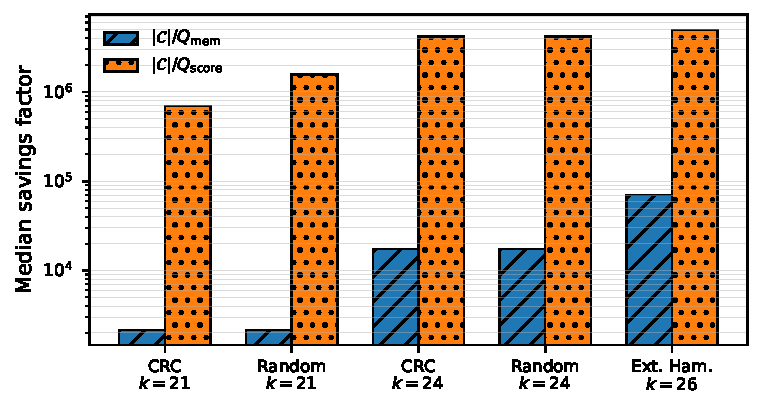
\includegraphics[width=\columnwidth]{figures/figure_query_savings.pdf}
\caption{Frozen $n=32$ median savings relative to codebook-wise work. Complete likelihood scoring
is reduced far more than membership queries because only discovered codewords are scored.}
\label{fig:savings}
\end{figure}

\subsection{What the savings do and do not show}
The distinct insertion-sphere generator attempted about $1.94\times$ fewer hypotheses than the
$2n$ history-pair generator, but its wall-clock advantage did not pass the preregistered gate.
Thus the classical $n+1$ generation result is retained as a clean implementation device, not a
latency contribution. Against the generic branch-and-bound implementation, FIBER was faster in four
of five $n=32$ cells and slower in several $n=24$ cells. The strongest practical statement is the
large reduction relative to exhaustive codeword-wise scoring and the competitive finite behavior
against this one generic exact search; no universal latency claim is made.

The sampled high-rate cells have high ML block-error rates. This does not indicate decoder failure:
all exact comparators agree on the ML result. It does limit system-performance interpretation, and
this paper therefore makes a decoder-complexity claim rather than a coding-gain claim.

\subsection{Best history versus aggregate ML}
The campaign recorded many cases in which a lexicographically selected first-shell representative
differed from the selected aggregate-ML representative, but the corresponding tie sets always
overlapped. The finite campaign therefore had no case where the first-shell codeword tie set was
disjoint from the aggregate-ML tie set. These representative differences are not used as evidence
of strict pathwise suboptimality; Theorem~\ref{thm:reversal} supplies a strict structural family.
A larger prevalence study would answer a different question and is not needed for exactness.

\section{Claim boundaries and conclusion}
The generic ideas of summing paths, threshold aggregation, membership-oracle decoding, and the
$n+1$ insertion-sphere cardinality are not claimed as new. The defensible contributions are the
strict channel/coding family, the exact shell-certified specialization, the stop/query theorem,
and the exact evidence separating membership, scoring, generation, and time. For a
one-deletion-plus-substitution channel, ranking histories and ranking candidate words are different
operations. FIBER-GRAND restores exact aggregate ML while retaining code membership as the code
interface. The stopping theorem gives a channel-specific query bound, and exact finite-length
evidence shows repeated reductions of several orders of magnitude in complete codeword scoring.
The current evidence supports a narrow Paper-I contribution. Before any submission claim, the proof
and novelty positioning require external proof and novelty review; no broader synchronization-channel
claim follows from this model.

\section*{Reproducibility statement}
All reported values are generated from immutable commit \texttt{\PhaseTwoCCommit}. The campaign
specification, exact C++ source, trial-level outputs, theorem checks, and manifests are retained in
the public research repository. Phase 2D introduces no new simulation.

\balance
\begin{thebibliography}{10}
\bibitem{duffy2019grand}
K.~R. Duffy, J.~Li, and M.~M\'edard, ``Capacity-achieving guessing random additive noise decoding,''
\emph{IEEE Trans. Inf. Theory}, vol.~65, no.~7, pp.~4023--4040, Jul.~2019,
doi: 10.1109/TIT.2019.2896110.

\bibitem{davey2001reliable}
M.~C. Davey and D.~J.~C. MacKay, ``Reliable communication over channels with insertions, deletions,
and substitutions,'' \emph{IEEE Trans. Inf. Theory}, vol.~47, no.~2, pp.~687--698, Feb.~2001,
doi: 10.1109/18.910582.

\bibitem{banerjee2022sequential}
A.~Banerjee, A.~Lenz, and A.~Wachter-Zeh, ``Sequential decoding of convolutional codes for
synchronization errors,'' in \emph{Proc. IEEE Inf. Theory Workshop (ITW)}, 2022, pp.~630--635,
doi: 10.1109/ITW54588.2022.9965844.

\bibitem{gabrys2023beyond}
R.~Gabrys, V.~Guruswami, J.~Ribeiro, and K.~Wu, ``Beyond single-deletion correcting codes:
Substitutions and transpositions,'' \emph{IEEE Trans. Inf. Theory}, vol.~69, no.~1, pp.~169--186,
Jan.~2023, doi: 10.1109/TIT.2022.3202856.

\bibitem{ozaydin2022optimal}
B.~Ozaydin, M.~M\'edard, and K.~R. Duffy, ``GRAND-assisted optimal modulation,'' in
\emph{Proc. IEEE GLOBECOM}, 2022, arXiv:2210.16187.

\bibitem{fagin2003optimal}
R.~Fagin, A.~Lotem, and M.~Naor, ``Optimal aggregation algorithms for middleware,''
\emph{J. Comput. Syst. Sci.}, vol.~66, no.~4, pp.~614--656, 2003,
doi: 10.1016/S0022-0000(03)00026-6.

\bibitem{sabary2022decoding}
O.~Sabary, D.~Bar-Lev, Y.~Gershon, A.~Yucovich, and E.~Yaakobi, ``On the decoding error weight of
one or two deletion channels,'' arXiv:2201.02466, 2022.

\bibitem{hoeffding1963probability}
W.~Hoeffding, ``Probability inequalities for sums of bounded random variables,''
\emph{J. Amer. Statist. Assoc.}, vol.~58, no.~301, pp.~13--30, 1963.
\end{thebibliography}
\end{document}
